\documentclass{article}
\usepackage{graphicx} % Required for inserting images
\usepackage{amsmath}
\usepackage{amssymb}
\usepackage{hyperref}
\usepackage{booktabs}
\usepackage{float}
\usepackage{parskip}
\usepackage{subcaption}

\setlength{\parindent}{0pt}
\setlength{\parskip}{0.5em}

\begin{document}

% --- Custom title page ---
\begin{titlepage}
    \centering
    \vspace*{\fill} % centers vertically

    {\Huge \textbf{Reproduction Report}} \\[3ex]  % Bigger title
    {\huge A Hierarchical Probabilistic U-Net} \\[10ex] % Subtitle, slightly smaller

    {\Large Divyashree Doddbele Aswatha Narayana} \\[2ex]

    {\large \today}

    \vspace*{\fill}
    \thispagestyle{empty} % no page number
\end{titlepage}

% --- Start the actual report from page 2 ---
\setcounter{page}{1}

\section{Introduction}
In medical imaging, scans often contain ambiguity. For example, in a lung CT scan, a lesion may look almost the same whether it is cancerous or not. This creates ambiguity because the same image can lead to multiple valid segmentations. Traditional segmentation models usually give only one output, which may hide these uncertainties and lead to wrong decisions in medical use.

The \textbf{Probabilistic U-Net (sPU-Net)}~\cite{Kohl2018} was proposed to solve this problem. It combines a U-Net~\cite{Ronneberger2015} with a conditional variational autoencoder (cVAE), so the model can generate many different but consistent segmentations. Later, the \textbf{Hierarchical Probabilistic U-Net (HPU-Net)}~\cite{Kohl2019} improved on this idea by introducing a hierarchy of latent variables. This hierarchy allows the model to capture both large global differences (like lesion presence) and small local details (like fuzzy edges). With this, the HPU-Net provides better results and a more realistic description of uncertainty in medical images.

In this report, we reproduce Figure 2 from the Hierarchical Probabilistic U-Net (HPU-Net) paper~\cite{Kohl2019}. The original figure is shown in Figure \ref{fig:lidc} for reference. The figure compares the Probabilistic U-Net (sPU-Net)~\cite{Kohl2018} and the HPU-Net on the LIDC-IDRI dataset. The original code released by the authors at DeepMind was written in TensorFlow,\footnote{\url{https://github.com/SimonKohl/probabilistic_unet}} while in this work the models were re-implemented in PyTorch \footnote{\url{https://github.com/divya-dan/HPU-Net}}to faithfully reproduce Figure 2 from the original work \footnote{\url{https://github.com/google-deepmind/deepmind-research/tree/master/hierarchical_probabilistic_unet}}. We trained both models using the setups described in the respective papers and present the results. The report covers dataset preparation, model architecture, training, and evaluation.

This report is organized as follows. Section~2 explains the models and the 
training details. Section~3 shows the reproduction results. Section~4 presents 
the conclusion and outlook. Section~5 gives acknowledgments and references.

\begin{figure}[tp]
\centering
%
\includegraphics[width=0.8\textwidth]{./figures/Figure_2.png}
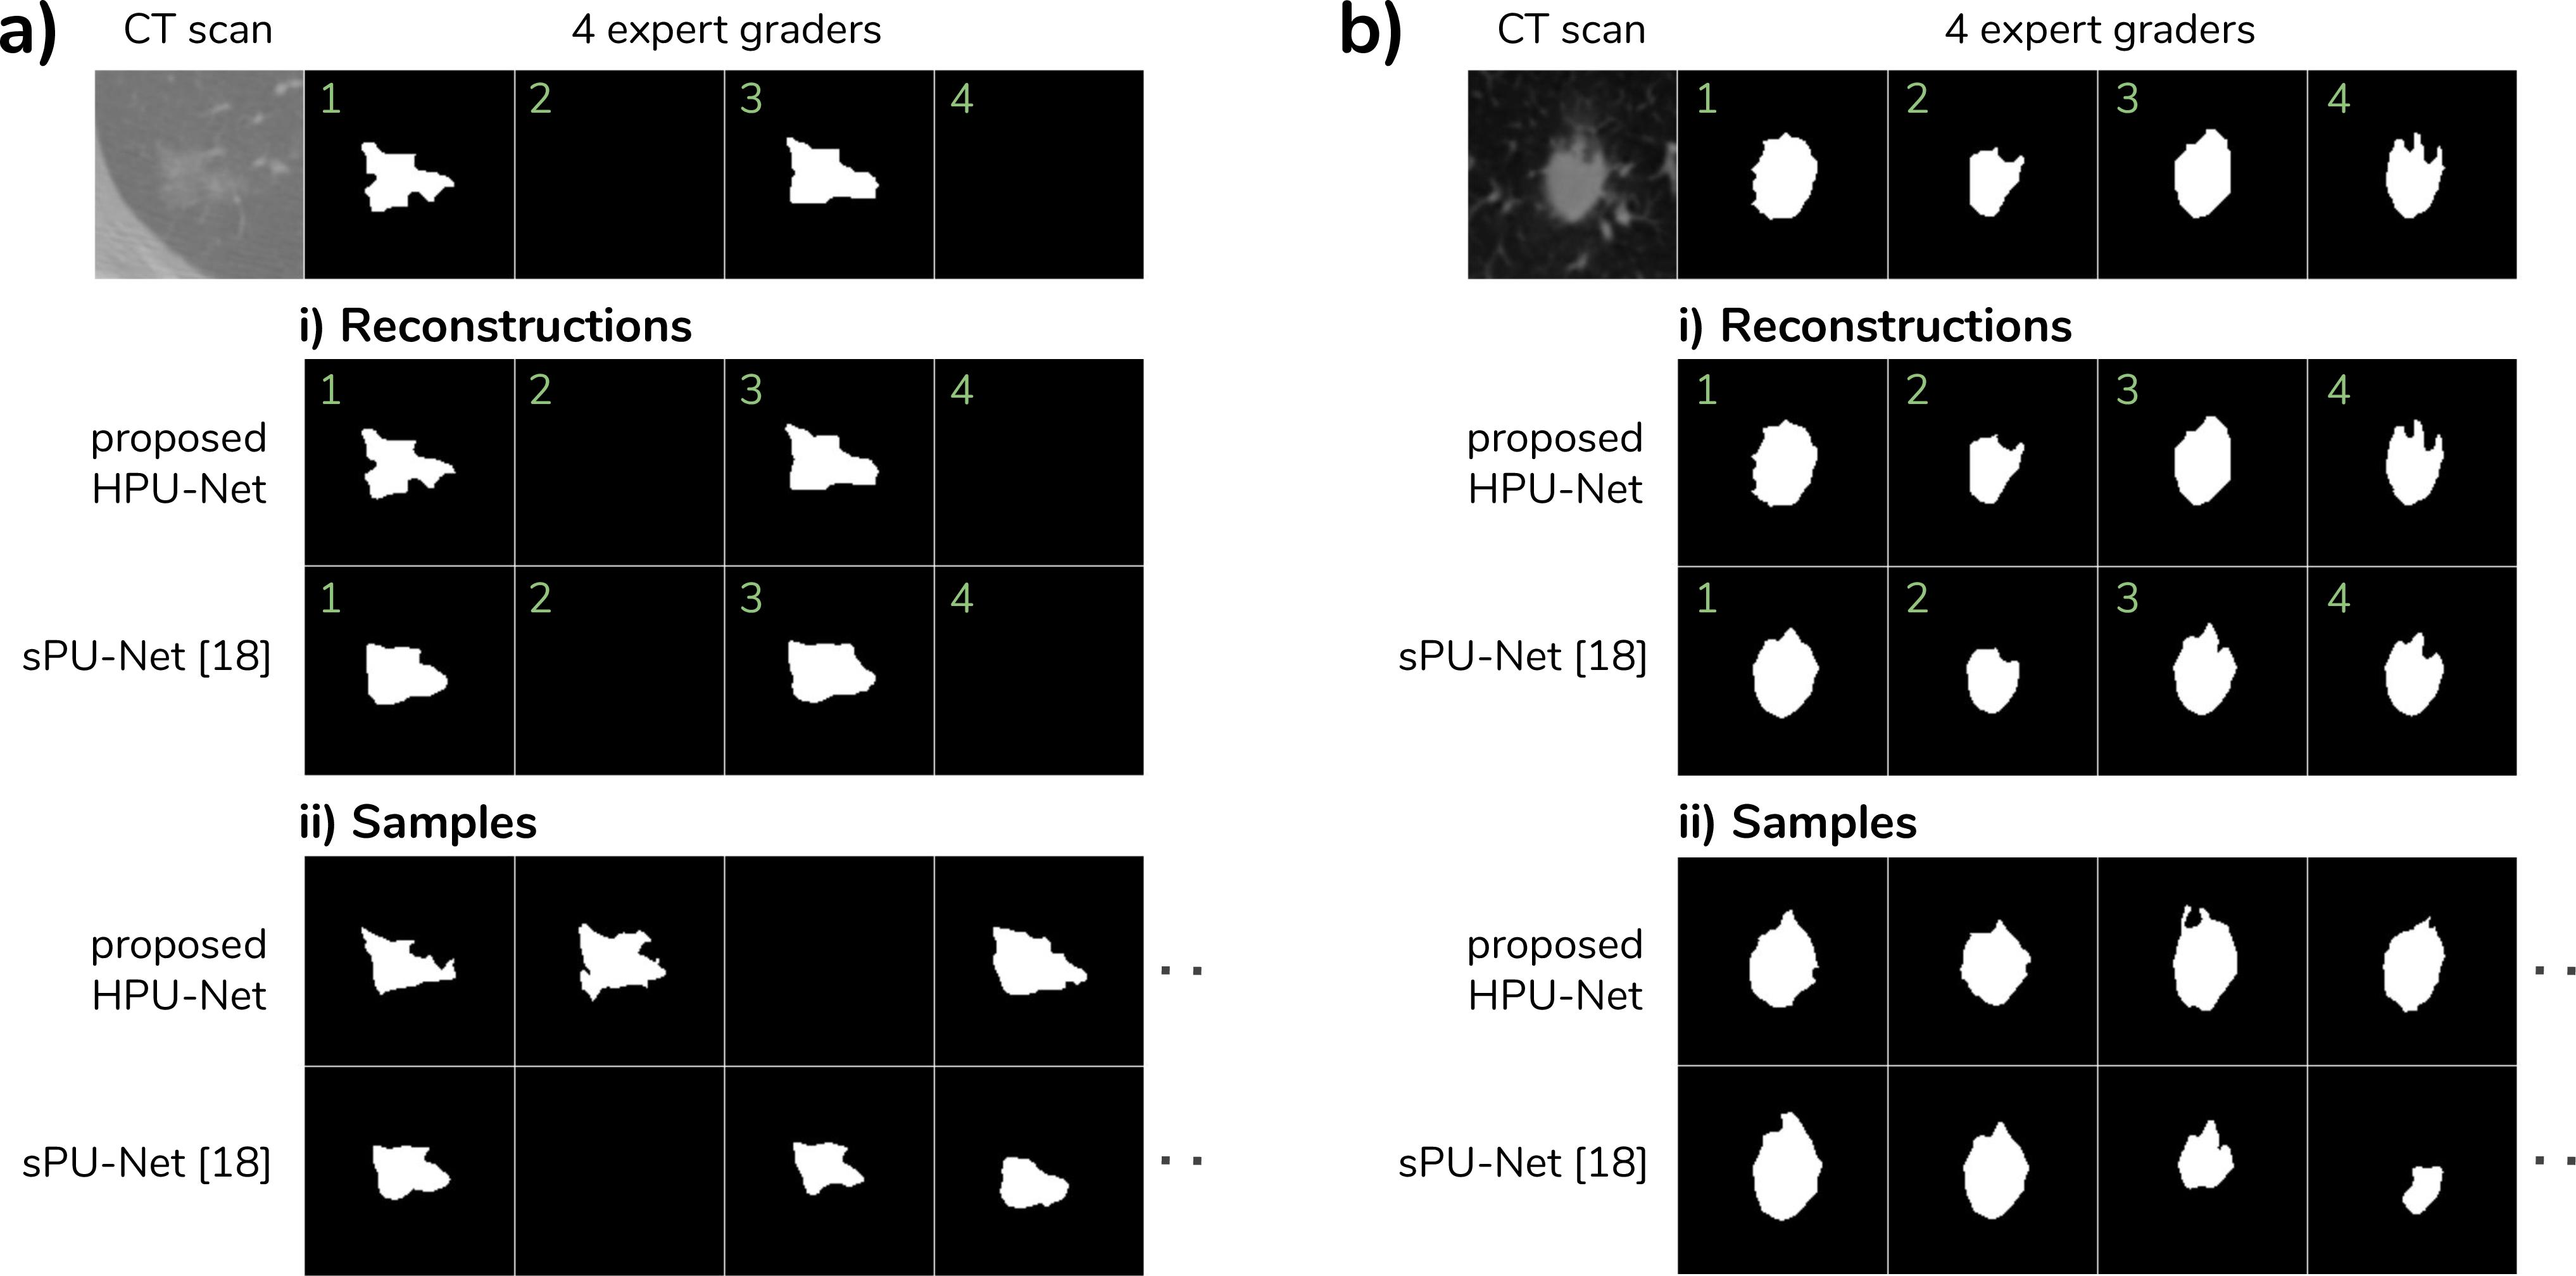
\includegraphics[width=0.95\textwidth]{Figure_2.jpg}
\caption{Two example CT scans with the 4 available expert gradings from LIDC-IDRI. (\textbf{i}) Reconstructions of the 4 graders and (\textbf{ii}) Sampled segmentations. Note that the gradings can be empty, as foreground annotations correspond to supposed abnormal cases only. Figure from~\cite{Kohl2019}.}
\label{fig:lidc}
\end{figure}

\section{Architecture and Training}

Both sPU-Net and HPU-Net are generative segmentation models that can produce 
multiple possible outputs for the same input image. They do this by sampling 
latent variables and then reconstructing the segmentation maps from them. 

\textbf{Sampling:}  
To generate a segmentation, the model samples latent variables from a prior 
distribution. The prior is modeled as a Gaussian, with mean and variance predicted 
from the input image~\cite{Kohl2018}. In the sPU-Net this is a single global latent 
vector, while the HPU-Net extends this idea with hierarchical latent maps~\cite{Kohl2019}. 

At each decoder scale, a latent map is sampled and concatenated with the decoder 
features before up-sampling and merging with encoder features. The higher-scale 
latents depend on both the image and the latents sampled at lower scales, forming 
a hierarchical prior. Each run of the network with a new sample produces a different 
but plausible segmentation, and only the decoder part needs to be rerun to generate 
multiple hypotheses for the same input image~\cite{Kohl2019}.

\textbf{Training:}  
Both sPU-Net and HPU-Net are trained using the variational autoencoder (VAE) framework, 
which maximizes the evidence lower bound (ELBO) on the likelihood of predicting the 
segmentation from the image~\cite{Kingma2014,Kohl2018}. In this setup, the model learns 
a posterior distribution that depends on both the input image and the ground-truth 
segmentation. During training, latent variables are sampled from this posterior and 
passed through the decoder to reconstruct the segmentation.  

The training loss has two parts: \\
1) a reconstruction loss, defined as cross-entropy between prediction and target,  \\
2) a Kullback–Leibler (KL) divergence, which encourages the posterior to be close to the prior~\cite{Kohl2019}.  

Unlike standard segmentation, the reconstruction error is summed over pixels before averaging across the batch, and then reported per pixel for comparability. 

Plain ELBO can lead to weak priors. To address this, the HPU-Net uses the GECO objective~\cite{Rezende2018}, which dynamically balances the reconstruction and KL terms. GECO sets a target reconstruction level \(\tau\) and update a Lagrange multiplier \(\lambda\) from an \textbf{exponential moving average} of the gap \(\mathbb{E}[L_{\text{rec}}]-\tau\) \([4]\).
Early on, this pushes the model to hit the target, then the emphasis shifts to the KL term, strengthening the prior.

Additionally, HPU-Net applies hard negative mining; Only the worst 2\% pixels
in each batch are used for backpropagation~\cite{Shrivastava2016}. This forces the model 
to focus on the most difficult pixels and improves segmentation performance.

In the sPU-Net, a separate prior network predicts the latent distribution. 
The HPU-Net removes this and instead uses U-Net features to predict the prior, which reduces parameters and speeds up training.

\subsection{Dataset}
The LIDC-IDRI dataset~\cite{Armato2011,Clark2013} contains 1018 lung CT scans from 1010 patients, with manual lesion segmentations provided by four experts. For the reproduction, we used the preprocessed version of this dataset available in a public Google Cloud Storage bucket\footnote{\url{https://console.cloud.google.com/storage/browser/hpunet-data/lidc_crops}}, which contains cropped images prepared for the HPU-Net experiments.

The preprocessed dataset was created following the setup in~\cite{Kohl2018}. The authors used annotations from a second reading and split the data into 722 patients for training, 144 for validation, and 144 for testing. Each scan was cropped into 2D images of size 180 x 180 pixels, resulting in 8882 training, 1996 validation, and 1992 test images. Crops were centered on positions where at least one grader marked a lesion. The preprocessing also filtered to include only lesions described as polygons in the XML files and larger than 3mm, since smaller ones are considered less relevant~\cite{Armato2011}. Inconsistent DICOM slices were filtered out, and masks from different graders were assumed to belong to the same lesion if their bounding boxes overlapped.

In this dataset, even empty masks are valid expert labels, so we treat IoU = 1 when the model correctly predicts the absence of a lesion. The reconstruction IoU (IoU$_{\text rec}$)  is averaged across all four graders.

\subsection{Training}

\textbf{Data augmentation:}   
During training~\cite{Kohl2019}, we apply random augmentations to both images and labels
($180 \times 180$ pixel tiles), including random elastic deformation, rotation, mirroring, shearing, scaling, and random translated crops, resulting in $128 \times 128$ tiles. Any padding introduced during augmentation is masked from the loss. 

\subsubsection{HPU-Net}
  
The HPU-Net~\cite{Kohl2019} is based on an 8-scale U-Net. Each stage of the encoder and decoder contains three pre-activated residual blocks with $3 \times 3$ convolutions. When the number of feature channels changes, a $1 \times 1$ convolution is used in the skip connection to keep the dimensions consistent.  

The images are reduced in size step by step using average pooling for down-sampling, and then enlarged again with nearest-neighbor interpolation for up-sampling. Skip connections link encoder and decoder features at every scale, so that fine image details from the encoder are carried over to the decoder.  

The model begins with 24 channels and doubles them at each down-sampling stage, up to a maximum of 192. The encoder compresses the input from $128 \times 128$ pixels down to a single $1 \times 1$ feature map, which encodes the global information of the image.  

In the decoder, a latent map is added at each of the 8 scales, from a global $1 \times 1$ level to a fine $128 \times 128$ level. This hierarchical design helps the model capture both large-scale uncertainties (for example, whether a lesion is present) and fine-scale details (such as fuzzy boundaries). To make training focus on the most difficult areas, only the hardest 2\% of pixels are backpropagated, selected stochastically using Gumbel sampling.  

\textbf{Training setup:}  
\begin{itemize}
  \item Batch size: 32
  \item Training steps: 240{,}000 iterations
  \item Optimizer: Adam with weight decay $1 \times 10^{-5}$
  \item Learning rate: $1 \times 10^{-4}$, reduced by factor of 0.5 at milestones 60{,}000, 120{,}000, 180{,}000, and 210{,}000 iterations
  \item Loss function: GECO objective with  
  \begin{itemize}
    \item reconstruction constraint $\kappa = 0.05$,  
    \item exponential moving average factor $\alpha = 0.99$,  
    \item initial multiplier $\lambda = 1.0$,  
    \item step size = 0.01.  
  \end{itemize}
\end{itemize}

\subsubsection{sPU-Net}
  
The sPU-Net~\cite{Kohl2018} is based on a 5-scale U-Net. Each block of the encoder and decoder has three $3 \times 3$ convolution layers with ReLU activations. Down-sampling and up-sampling are done with bilinear interpolation, and skip connections link encoder and decoder features so that spatial details are preserved.  

The network starts with 32 channels, doubling at each stage up to 512 at the bottleneck. At this bottleneck, a single \emph{global latent vector with six dimensions} is sampled. The latent distribution is predicted by two networks: a prior network, which depends only on the input image, and a posterior network, which depends on both the image and the ground-truth segmentation.  

The latent vector is broadcast to match the decoder resolution, concatenated with decoder features, and passed through a sequence of $1 \times 1$ convolutions to produce the final segmentation map. 

\textbf{Training setup:}
\begin{itemize}
  \item Batch size: 32
  \item Training steps: 240,000 iterations
  \item Optimizer: Adam with weight decay $1 \times 10^{-5}$
  \item Learning rate: $1 \times 10^{-4}$, reduced by factor of 0.5 at milestones 48{,}000, 96{,}000, 144{,}000, 192{,}000 and 216{,}000 iterations
  \item Loss: Standard ELBO with $\beta = 1$:
  \[
    \mathcal{L} = \text{Reconstruction BCE} + \text{KL divergence}
  \]
  The reconstruction loss is summed over pixels, averaged per image, and then averaged across the batch.
\end{itemize}

\vspace{1ex}

\section{Results}
The original HPU-Net paper reports that the Hierarchical Probabilistic U-Net (HPU-Net) performs better than the standard Probabilistic U-Net (sPU-Net) in both reconstruction fidelity and Hungarian matched IOU ~\cite{Kohl2019}. The hierarchical latent scales of HPU-Net capture lesions more precisely and preserve fine details, while sPU-Net’s global latent vector often produces coarser, blob-like segmentations. This difference is also visible in our reproduced results (Figure~\ref{fig:results}), where HPU-Net provides sharper boundaries and more realistic variability in comparison with sPU-Net.

\begin{table}[H]
\centering
\caption{Comparison of evaluation metrics between original paper and reproduced results.}
\label{tab:metrics}
\begin{tabular}{|r||l|l|l|}
\hline
\textbf{Model} & \textbf{IoU\textsubscript{rec}} & \textbf{Hungarian-} & \textbf{GED\textsuperscript{2}} \\
& & \textbf{matched IoU} & \\
\hline
\hline
sPU-Net & $0.75 \pm 0.04$ & $0.50 \pm 0.03$ & $0.32 \pm 0.03$ \\
(paper) & & & \\
\hline
sPU-Net & $0.76 \pm 0.15$ & $0.47 \pm 0.23$ & $0.44 \pm 0.38$ \\
(reproduced) & & & \\
\hline
HPU-Net & $0.97 \pm 0.00$ & $0.53 \pm 0.01$ & $0.27 \pm 0.01$ \\
(paper) & & & \\
\hline
HPU-Net & $0.95 \pm 0.07$ & $0.49 \pm 0.20$ & $0.39 \pm 0.29$ \\
(reproduced) & & & \\
\hline
\end{tabular}
\end{table}

\begin{figure}[H]
    \centering
    \begin{subfigure}{\textwidth}
        \centering
        
\includegraphics[width=0.78\textwidth]{comparative_row_00000.png}
        \caption{Sample 1.}
        \label{fig:results_1}
    \end{subfigure}
    
    \vspace{0.2cm} % Add some vertical space between the two images
    
    \begin{subfigure}{\textwidth}
        \centering
        
\includegraphics[width=0.78\textwidth]{comparative_row_00001.png}
        \caption{Sample 2.}
        \label{fig:results_2}
    \end{subfigure}
    
    \caption{Here we show comparison of sPU-Net and HPU-Net. For each sample, top row shows the original CT scan and four expert grader annotations. The middle rows show model reconstructions attempting to match each expert grader, with IoU scores indicating reconstruction quality. The bottom rows show samples generated by each model.}
    \label{fig:results}
\end{figure}

Table~\ref{tab:metrics} compares the reproduction metrics on LIDC - IDRI dataset with the metrics reported in the paper. The metrics include:  
\begin{itemize}
    \item \textbf{Reconstruction IoU (IoU\textsubscript{rec})}, which measures how well the model can reconstruct a given expert segmentation.  
    \item \textbf{Hungarian-matched IoU}, which evaluates how well the model samples align with the expert annotations after optimal matching~\cite{Kuhn1955, Munkres1957}.  
    \item \textbf{Generalized Energy Distance (GED\textsuperscript{2})}, which measures how well the conditional distribution produced by a generative model agrees with the given ground-truth distribution~\cite{Kohl2019}.  
\end{itemize}

Both the original results and our reproduction confirm the same trend: HPU-Net outperforms sPU-Net in all evaluation metrics.

\section{Conclusion and Outlook}

This work reproduced Figure~2 from the HPU-Net paper and showed that the 
HPU-Net performs better than the sPU-Net on the LIDC-IDRI dataset. The results 
support the idea that adding hierarchical latent variables improves both 
reconstruction quality and the modeling of uncertainty. 



As future work, the same setup can be tested on other datasets such as SNEMI3D 
or Cityscapes. It can also be extended by trying different numbers of latent 
scales or other training objectives to study their effect on segmentation 
quality and uncertainty. The code and setup used here can be reused and adapted 
for such experiments on other medical imaging datasets.


\section{Acknowledgement}
We would like to thank the authors of the Probabilistic U-Net~\cite{Kohl2018} and Hierarchical Probabilistic U-Net~\cite{Kohl2019} papers for making their work available. I also acknowledge the LIDC-IDRI dataset~\cite{Armato2011,Clark2013}, which made this reproduction possible.

\bibliographystyle{plain}
\begin{thebibliography}{10}

\bibitem{Kohl2018}
S. A. A. Kohl, B. Romera-Paredes, C. Meyer, J. De Fauw, J. Ledsam, K. Maier-Hein, S. Eslami, D. J. Rezende, and O. Ronneberger.  
\newblock A Probabilistic U-Net for Segmentation of Ambiguous Images.  
\newblock In \emph{Advances in Neural Information Processing Systems (NeurIPS)}, 2018.

\bibitem{Kohl2019}
S. A. A. Kohl, B. Romera-Paredes, K. Maier-Hein, D. J. Rezende, S. Eslami, P. Kohli, A. Zisserman, and O. Ronneberger.  
\newblock A Hierarchical Probabilistic U-Net for Modeling Multi-Scale Ambiguities.  
\newblock arXiv preprint arXiv:1905.13077, 2019.

\bibitem{Ronneberger2015}
O. Ronneberger, P. Fischer, and T. Brox.  
\newblock U-Net: Convolutional Networks for Biomedical Image Segmentation.  
\newblock In \emph{MICCAI}, 2015.

\bibitem{Rezende2018}
D. J. Rezende and F. Viola.  
\newblock Taming VAEs.  
\newblock arXiv preprint arXiv:1810.00597, 2018.

\bibitem{Armato2011}
S. G. Armato et al.  
\newblock The Lung Image Database Consortium (LIDC) and Image Database Resource Initiative (IDRI).  
\newblock \emph{Medical Physics}, 38(2):915–931, 2011.

\bibitem{Clark2013}
K. Clark et al.  
\newblock The Cancer Imaging Archive (TCIA): Maintaining and Operating a Public Information Repository.  
\newblock \emph{Journal of Digital Imaging}, 26(6):1045–1057, 2013.

\bibitem{Kingma2014}
D. P. Kingma and M. Welling.  
\newblock Auto-Encoding Variational Bayes.  
\newblock In \emph{International Conference on Learning Representations (ICLR)}, 2014.

\bibitem{Shrivastava2016}
A. Shrivastava, A. Gupta, and R. Girshick.  
\newblock Training region-based object detectors with online hard example mining.  
\newblock In \emph{Proceedings of the IEEE Conference on Computer Vision and Pattern Recognition (CVPR)}, pages 761–769, 2016.

\bibitem{Kuhn1955}
H. W. Kuhn.  
\newblock The Hungarian method for the assignment problem.  
\newblock \emph{Naval Research Logistics Quarterly}, 2(1--2):83--97, 1955.

\bibitem{Munkres1957}
J. Munkres.  
\newblock Algorithms for the assignment and transportation problems.  
\newblock \emph{Journal of the Society for Industrial and Applied Mathematics}, 5(1):32--38, 1957.



\end{thebibliography}

\end{document}